\documentclass[border=2pt,12pt]{standalone}
\usepackage[T1]{fontenc}
\usepackage{mathptmx}
\usepackage{tikz}
\usetikzlibrary{arrows.meta,positioning,calc}
\tikzset{
  bloco/.style={draw, rounded corners=2pt, minimum height=8mm, minimum width=17mm,
                align=center, font=\small, fill=white, inner sep=2pt},
  soma/.style={draw, circle, inner sep=0pt, minimum size=5mm, font=\small, fill=white},
  seta/.style={-{Stealth[length=2mm]}, thick},
  rotulo/.style={font=\small},
}
\begin{document}
% Figura 4: s(n) = x1(n) + mu m(n) (eq. 8); s(n) realimenta o mapa do transmissor.
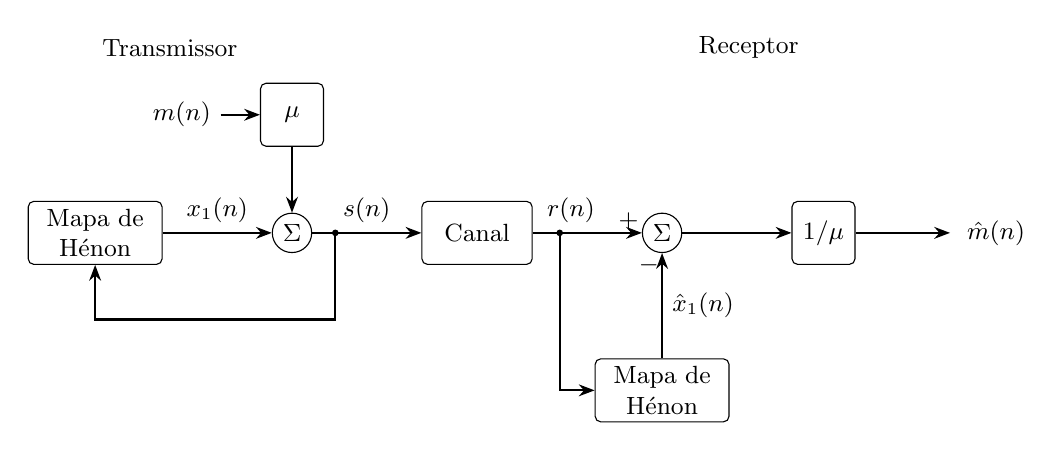
\begin{tikzpicture}
\node[bloco] (mapa)  at (0,0)     {Mapa de\\Hénon};
\node[soma]  (soma)  at (2.5,0)   {$\Sigma$};
\node[bloco, minimum width=8mm] (mu) at (2.5,1.5) {$\mu$};
\node[rotulo] (m)    at (1.1,1.5) {$m(n)$};
\node[bloco, minimum width=14mm] (canal) at (4.85,0) {Canal};
\node[soma]  (sub)   at (7.2,0)   {$\Sigma$};
\node[bloco] (copia) at (7.2,-2.0) {Mapa de\\Hénon};
\node[bloco, minimum width=8mm] (inv) at (9.25,0) {$1/\mu$};
\node[rotulo, anchor=west] (mh) at (10.95,0) {$\hat m(n)$};

\draw[seta] (mapa) -- node[above, rotulo]{$x_1(n)$} (soma);
\draw[seta] (m) -- (mu);
\draw[seta] (mu) -- (soma);
\draw[seta] (soma) -- node[above, rotulo]{$s(n)$} (canal);
\draw[seta] (canal) -- node[above, rotulo, pos=0.35]{$r(n)$} (sub);
% realimentação de s(n) para o mapa
\coordinate (fb) at (3.05,0);
\fill (fb) circle (1.2pt);
\draw[seta] (fb) -- (3.05,-1.1) -- (0,-1.1) -- (mapa.south);
% r(n) desce fora da caixa e entra pela lateral esquerda da cópia
\coordinate (rc) at (5.9,0);
\fill (rc) circle (1.2pt);
\draw[seta] (rc) -- (5.9,-2.0) -- (copia.west);
\draw[seta] (copia) -- node[right, rotulo]{$\hat x_1(n)$} (sub);
\draw[seta] (sub) -- (inv);
\draw[seta] (inv.east) -- ++(1.2,0);
% sinais do somador do receptor, cada um do lado da sua seta
\node[rotulo, anchor=south east, inner sep=1pt] at (sub.west) {$+$};
\node[rotulo, anchor=north east, inner sep=1pt] at (sub.south) {$-$};
\node[rotulo] at (0.95,2.35) {Transmissor};
\node[rotulo] at (8.3,2.35) {Receptor};
\end{tikzpicture}
\end{document}
